\section{Experimentaci'on}

\subsection{Resultados}

Comparamos una implementaci'on en C, con la vectorizada\footnote{El c'odigo de ambas se puede encontrar en \url{https://github.com/guidotag/Image-Morphing}.}. Para esto, tomamos dos imagenes de tama\~{n}o $1024 \times 768$, y trazamos 44 segmentos sobre cada una de ellas. En la figura \ref{fig2} se puede ver la metamorfosis utilizando los 44 segmentos.

Para la comparaci'on, decidimos dejar fijas las im'agenes origen y destino, es decir que $w = 1024$ y $h = 768$, fijar la cantidad de frames de la metamorfosis en $f = 100$, y s'olo variar la cantidad de segmentos $s$ utilizados. Esta elecci'on se basa en que el par'ametro $s$ es el que determina la intensidad del c'omputo de cada una de las llamadas individuales a la implementaci'on del algoritmo \ref{algo1}, que es la pieza que hemos vectorizado. Los par'ametros $f$, $w$ y $h$ solamente marcan cu'antas veces se llama a ese procedimiento.

Para cada una de las implementaciones, variando $s \in \{0, 5, 10, 15, 20, 25, 30, 35, 40\}$, medimos el tiempo de ejecuci'on total del algoritmo \ref{algo2}. Esto incluye el overhead que impone el framework utilizado para la escritura de los frames del video a lo largo de todo el proceso, al finalizar cada iteraci'on. Como veremos a continuaci'on, este overhead es despreciable respecto del resto del procesamiento.

En la figura \ref{fig8} presentamos los resultados de la comparaci'on. Ambas versiones fueron compiladas mediante la herramienta de Intel, cuyo grado de optimizaci'on es mucho mayor que otros compiladores, como GCC. Adem'as se utiliz'o el flag -O3, la opci'on de optimizaci'on m'as agresiva. Medimos el tiempo de ejecuci'on en cantidad de ciclos de reloj, utilizando el registro TSC (Time Stamp Counter) de un procesador Intel\textregistered Core\texttrademark i5-3470 compuesto de cuatro cores de 3.20GHz cada uno.

Recordemos que el costo del algoritmo \ref{algo2} es proporcional a $f \times w \times h \times s$, de modo que el gr'afico de tiempo de ejecuci'on en funci'on de $s$ ser'a una recta con pendiente proporcional a $f \times w \times h$.

\begin{figure}[H]
	\begin{center}
		% GNUPLOT: LaTeX picture with Postscript
\begingroup
  \makeatletter
  \providecommand\color[2][]{%
    \GenericError{(gnuplot) \space\space\space\@spaces}{%
      Package color not loaded in conjunction with
      terminal option `colourtext'%
    }{See the gnuplot documentation for explanation.%
    }{Either use 'blacktext' in gnuplot or load the package
      color.sty in LaTeX.}%
    \renewcommand\color[2][]{}%
  }%
  \providecommand\includegraphics[2][]{%
    \GenericError{(gnuplot) \space\space\space\@spaces}{%
      Package graphicx or graphics not loaded%
    }{See the gnuplot documentation for explanation.%
    }{The gnuplot epslatex terminal needs graphicx.sty or graphics.sty.}%
    \renewcommand\includegraphics[2][]{}%
  }%
  \providecommand\rotatebox[2]{#2}%
  \@ifundefined{ifGPcolor}{%
    \newif\ifGPcolor
    \GPcolorfalse
  }{}%
  \@ifundefined{ifGPblacktext}{%
    \newif\ifGPblacktext
    \GPblacktexttrue
  }{}%
  % define a \g@addto@macro without @ in the name:
  \let\gplgaddtomacro\g@addto@macro
  % define empty templates for all commands taking text:
  \gdef\gplbacktext{}%
  \gdef\gplfronttext{}%
  \makeatother
  \ifGPblacktext
    % no textcolor at all
    \def\colorrgb#1{}%
    \def\colorgray#1{}%
  \else
    % gray or color?
    \ifGPcolor
      \def\colorrgb#1{\color[rgb]{#1}}%
      \def\colorgray#1{\color[gray]{#1}}%
      \expandafter\def\csname LTw\endcsname{\color{white}}%
      \expandafter\def\csname LTb\endcsname{\color{black}}%
      \expandafter\def\csname LTa\endcsname{\color{black}}%
      \expandafter\def\csname LT0\endcsname{\color[rgb]{1,0,0}}%
      \expandafter\def\csname LT1\endcsname{\color[rgb]{0,1,0}}%
      \expandafter\def\csname LT2\endcsname{\color[rgb]{0,0,1}}%
      \expandafter\def\csname LT3\endcsname{\color[rgb]{1,0,1}}%
      \expandafter\def\csname LT4\endcsname{\color[rgb]{0,1,1}}%
      \expandafter\def\csname LT5\endcsname{\color[rgb]{1,1,0}}%
      \expandafter\def\csname LT6\endcsname{\color[rgb]{0,0,0}}%
      \expandafter\def\csname LT7\endcsname{\color[rgb]{1,0.3,0}}%
      \expandafter\def\csname LT8\endcsname{\color[rgb]{0.5,0.5,0.5}}%
    \else
      % gray
      \def\colorrgb#1{\color{black}}%
      \def\colorgray#1{\color[gray]{#1}}%
      \expandafter\def\csname LTw\endcsname{\color{white}}%
      \expandafter\def\csname LTb\endcsname{\color{black}}%
      \expandafter\def\csname LTa\endcsname{\color{black}}%
      \expandafter\def\csname LT0\endcsname{\color{black}}%
      \expandafter\def\csname LT1\endcsname{\color{black}}%
      \expandafter\def\csname LT2\endcsname{\color{black}}%
      \expandafter\def\csname LT3\endcsname{\color{black}}%
      \expandafter\def\csname LT4\endcsname{\color{black}}%
      \expandafter\def\csname LT5\endcsname{\color{black}}%
      \expandafter\def\csname LT6\endcsname{\color{black}}%
      \expandafter\def\csname LT7\endcsname{\color{black}}%
      \expandafter\def\csname LT8\endcsname{\color{black}}%
    \fi
  \fi
  \setlength{\unitlength}{0.0500bp}%
  \begin{picture}(6802.00,3968.00)%
    \gplgaddtomacro\gplbacktext{%
      \csname LTb\endcsname%
      \put(1474,704){\makebox(0,0)[r]{\strut{} 0}}%
      \put(1474,1204){\makebox(0,0)[r]{\strut{} 5e+11}}%
      \put(1474,1704){\makebox(0,0)[r]{\strut{} 1e+12}}%
      \put(1474,2204){\makebox(0,0)[r]{\strut{} 1.5e+12}}%
      \put(1474,2703){\makebox(0,0)[r]{\strut{} 2e+12}}%
      \put(1474,3203){\makebox(0,0)[r]{\strut{} 2.5e+12}}%
      \put(1474,3703){\makebox(0,0)[r]{\strut{} 3e+12}}%
      \put(1606,484){\makebox(0,0){\strut{} 0}}%
      \put(2206,484){\makebox(0,0){\strut{} 5}}%
      \put(2806,484){\makebox(0,0){\strut{} 10}}%
      \put(3406,484){\makebox(0,0){\strut{} 15}}%
      \put(4006,484){\makebox(0,0){\strut{} 20}}%
      \put(4605,484){\makebox(0,0){\strut{} 25}}%
      \put(5205,484){\makebox(0,0){\strut{} 30}}%
      \put(5805,484){\makebox(0,0){\strut{} 35}}%
      \put(6405,484){\makebox(0,0){\strut{} 40}}%
      \put(176,2203){\rotatebox{-270}{\makebox(0,0){\strut{}TSC}}}%
      \put(4005,154){\makebox(0,0){\strut{}Cantidad de segmentos ($s$)}}%
    }%
    \gplgaddtomacro\gplfronttext{%
      \csname LTb\endcsname%
      \put(5418,3530){\makebox(0,0)[r]{\strut{}C}}%
      \csname LTb\endcsname%
      \put(5418,3310){\makebox(0,0)[r]{\strut{}SIMD}}%
    }%
    \gplbacktext
    \put(0,0){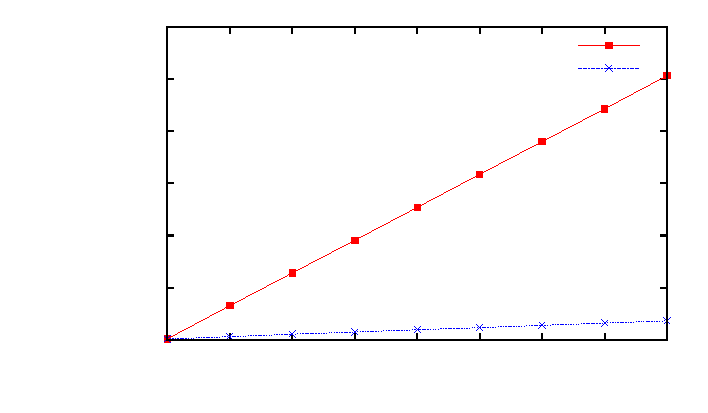
\includegraphics{texplots/morph_1024_768}}%
    \gplfronttext
  \end{picture}%
\endgroup

	\end{center}		
	\caption{Comparaci'on C vs. SIMD}
	\label{fig8}
\end{figure}

La siguiente tabla muestra los tiempos de ejecuci'on exactos, permitiendo calcular la diferencia de tiempo entre las implementaciones.

\begin{center}
\begin{tabular}{|c|c|c|c|}
\hline
$s$ & \textbf{C} & \textbf{SIMD} & \textbf{C / SIMD}\\
\hline
0 & 7309812582 & 5941940863 & 1.23\\
5 & 326478638311 & 29467020103 & 11.08\\
10 & 639832096193 & 52546672036 & 12.18\\
15 & 954306269556 & 73077639985 & 13.06\\
20 & 1269998392581 & 96104580737 & 13.21\\
25 & 1587171271314 & 116337177498 & 13.64\\
30 & 1901684635986 & 138126686002 & 13.77\\
35 & 2216291340338 & 160337691233 & 13.82\\
40 & 2535347665489 & 182194876866 & 13.91\\
\hline
\end{tabular} 
\end{center}

En el caso $s = 0$ se escribe el video casi sin realizar c'omputos durante el algoritmo \ref{algo1}, por lo que es una buena medida del overhead que impone el procesamiento de video. Observemos que el tiempo en ese caso es del orden de $10^{10}$ ciclos de clock, mientras que para $s > 0$ todos los valores van de los $10^{12}$ a los $10^{13}$ ciclos, es decir, de 100 a 1000 veces m'as. Esto indica que el overhead en cuesti'on va del 1\% al $0.1\%$, una cantidad despreciable de trabajo del procesador.

Como se ve, la implementaci'on SIMD es, a medida que $s$ crece, casi 14 veces m'as r'apida. Si bien la velocidad de crecimiento de la raz'on de los tiempos disminuye dr'asticamente a partir de $s = 15$, no se ve un estancamiento total de dicho valor, con lo cual podr'ia seguir increment'andose para valores de $s$ m'as grandes que 40. En este trabajo no exploraremos qu'e sucede m'as all'a de $s = 40$, pues no son valores de inter'es pr'actico.

\subsection{An'alisis}

En general, al vectorizar procedimientos obtenemos ganancias m'ultiplo de la cantidad de datos procesados al mismo tiempo. Sin embargo, en este caso, la vectorizaci'on supera ampliamente esa expectativa, al ser 14 veces m'as r'apida, pese a que cada ejecuci'on procesa s'olo 4 pixeles en paralelo. En busca de una explicaci'on para este fen'omeno, comparamos con lupa ambas implementaciones.

La implementaci'on con extensiones SIMD tiene dos caracter'isticas remarcables, directamente relacionadas con su performance:

\begin{itemize}
	\item \textbf{Casi todas las magnitudes involucradas se mantienen, todo el tiempo, en registros.} Esto permite evitar accesos a memoria, que son m'as de 100 veces m'as costosos que los accesos a registros, en el caso de un cache miss.
	\item \textbf{Todas las funciones auxiliares est'an implementadas en forma de macros.} Si bien esto permite reducir el overhead de una implementaci'on que usa etiquetas e instrucciones \texttt{call}, la motivaci'on verdadera fue hacer la programaci'on m'as sencilla, puesto que, en el intento de mantener la mayor'ia de los datos en registros, 'estos deb'ian ser manipulados cuidadosamente. Utilizando macros podemos decidir exactamente qu'e registros queremos que sean utilizados por una rutina.
\end{itemize}

Ambas caracter'isticas tienen desventajas. Por un lado, al intentar explotar al m'aximo la utilizaci'on de los registros, se hace mucho m'as complicada la programaci'on, al ser limitada la cantidad de registros que tenemos a nuestra disposici'on. Sortear este problema es simplemente una cuesti'on de planificar bien el programa. Por otro lado, la utilizaci'on de macros tiene dos desventajas. Primero, no es posible una utilizaci'on din'amica del c'odigo de la macro, en el sentido de que cada invocaci'on a ella replicar'a su c'odigo, haciendo que el c'odigo objeto de todo el programa sea mucho m'as largo. En nuestro caso, el c'odigo objeto de la vectorizaci'on consta de algunas cientos de l'ineas, de modo que no resulta una verdadera contra. En segundo lugar, no es posible depurar las l'ineas que componen a la macro, haciendo m'as dif'icil la detecci'on y correcci'on de errores.

Para realizar un an'alisis detallado de la versi'on C, hicimos un dump de su c'odigo objeto, siendo dos las observaciones que se desprenden del mismo:

\begin{itemize}
	\item \textbf{La cantidad neta de l'ineas del reverse mapping y todas las funciones auxiliares utilizadas, es de 750 l'ineas.} Esto es m'as del doble del tama\~{n}o de la versi'on SIMD, que tiene alrededor de 350. Si bien un programa m'as compacto no es necesariamente mejor, en este caso tenemos 350 l'ineas que fueron cuidadosamente pensadas, contrariamente a las 750 elaboradas por un compilador, lo cual podr'ia indicar que la mano humana est'a haciendo una diferencia.
	
	\item \textbf{Casi todas las variables locales involucradas en el ciclo principal del algoritmo fueron almacenadas en stack.} Esto obliga a hacer lecturas de memoria en cada llamada a una funci'on auxiliar, y escrituras de memoria para almacenar su resultado. Resulta claro el contraste con la implementaci'on en SIMD, en la que se busc'o mantener todos los datos que fueran posibles en los registros.
\end{itemize}

Como se puede ver, la diferencia que parece estar inclinando la balanza a favor de la versi'on SIMD (a'un m'as de lo que ya lo hace la vectorizaci'on) es el predominante uso de la memoria principal de la versi'on C. Para corroborar este hecho y comparar otras m'etricas de performance, realizamos un an'alisis con la herramienta \textit{perf} de Linux. Tomamos el caso $s = 20$ y corrimos el programa completo, una vez utilizando la implementaci'on en C, y otra con el procedimiento SIMD. Los resultados fueron los siguientes:

\begin{center}
\begin{tabular}{|l|c|c|}
\hline
& \textbf{C} & \textbf{SIMD}\\
\hline
\textbf{Ciclos de clock} & $1.43 \times 10^{12}$ & $1.07 \times 10^{11}$\\
\textbf{Instrucciones} & $9.69 \times 10^{11}$ & $2.03 \times 10^{11}$\\
\textbf{Instrucciones por ciclo} & $0.68$ & $1.90$\\
\textbf{Referencias a cache} & $1.96 \times 10^{7}$ & $1.87 \times 10^{7}$\\
\textbf{Cache misses} & $61.55$\% & $68.20$\%\\
\textbf{Branches} & $1.20 \times 10^{11}$ & $1.22 \times 10^{9}$\\
\textbf{Branch misses} & $0.60$\% & $0.73$\%\\
\textbf{Lecturas de memoria} & $2.70 \times 10^{9}$ & $4.17 \times 10^{8}$\\                                                    \textbf{Escrituras de memoria} & $1.99 \times 10^{11}$ & $5.50 \times 10^{9}$\\
\hline
\end{tabular}
\end{center}

Los n'umeros confirman que la cantidad de accesos a memoria de la implementaci'on SIMD es 'ordenes de magnitud menor. A esto se suma que la vectorizaci'on aprovecha mucho m'as al procesador, al ejecutar casi el triple de instrucciones por ciclo que la implementaci'on en C. Por 'ultimo, es remarcable la diferencia en la cantidad de branches (instrucciones de salto ejecutadas) que resulta 100 veces menor en la vectorizaci'on, siendo el porcentaje de errores de predicci'on aproximadamente el mismo, con lo cual, en total, la cantidad de errores de predicci'on tambi'en es 100 veces menor en la vectorizaci'on.